%!TEX root = ../thesis.tex
%*******************************************************************************
%*********************************** Sixth Chapter *****************************
%*******************************************************************************

\chapter{Research of the shape changes of the arterial pulses during proximal occlusions}  %Title of the First Chapter
\label{chapter apa}

\ifpdf
\graphicspath{{Chapter8/Figs/Raster/}{Chapter8/Figs/PDF/}{Chapter8/Figs/}}
\else
\graphicspath{{Chapter8/Figs/Vector/}{Chapter8/Figs/}}
\fi

The arterial pulses amplitude (APA) are the dynamic component of the impedance plethysmography signal. It lies within the basal impedance which represents about \SI{0.1}{\percent} of the total waveform \cite{anderson1984impedance}. Acquiring these signals can be quite challenging as noise levels could be higher than the actual signal making tough to isolate this waveform. However, obtaining this data provides valuable information about haemodynamics per heartbeat. It has been demonstrated that the shape of the waveform is an indicator of haemodynamic problems in the peripheral circulation. In this chapter, the analysis of the signals aims to differentiate morphological changes between baseline signals and the ones during venous, partial arterial and total occlusion.

As it has been described in the previous chapter, there is a shift in the impedance's baseline during each occlusion. However, it is desirable to study the effect that the different kind occlusions of the upper arm produce in the plethysmography waveforms.  This information may provide clues whether an occlusion may be occurring in either the venous or arterial circulation.  The designed iPG device supplies an output port denominated $Z_{AC}$ \mynote{To double check if this is the correct port name from the initial description} which provides a high-resolution view of the arterial pulses waveform.  In fact, as shown in the design section \ref{section design 1.5}, the signal was filtered and amplified nearly 2500 times to achieve this level of detail. Hence, the waveform obtained provides more in-depth detail and also improves the noise rejection of the signal.

The device produced an excellent result regarding filtering and isolation of the APA waveform. However, undoubtedly some of the noise was also amplified by the hardware. Therefore, further post-processing was required to clean up the plethysmography signal completely. Tighter filters (see table \ref{table:filters}) were applied to remove high and low frequency components. Also, the lower envelope component was also removed and levelled to zero.

The APA waveform produced by the device is inverted as represented by various other plethysmography method such as photoplethysmography. During the systolic cycle, the blood vessels expand allowing more blood volume. Hence, the impedance drops proportionally to the amount of blood because the forearm's segment is more electrically conductive. On the other hand, during the diastolic cycle, blood vessels empty causing a reduction the quantity of blood contained in the segment. As a result, the impedance increases.

The analysis of the plethysmographic wave was performed by averaging the waveforms detected using specialized algorithms able to identify an APA signal. The following section discusses the change of wave shape from a non-occlusion state to an occluded one. At the end of the section, the results of all participants are summarised \mynote{I could add a description of how the signal looks. For instance by adding 10 or 20 beats to show how the device worked.}

%%********************************** % Section 8.1 ******************************************
\section{Dataset for the arterial amplitude analysis}
\label{section apa 1}
The isolated APA waveforms reproduce the change of volume per heart beat within the sensing electrodes of the iPG device placed in the forearm. The filling of the vessels with blood produces small changes in resistivity that vary with the circulatory cycle (see section \ref{section impedance 9.1}), describing different peaks during a heart cycle.

\begin{figure}[!htpb]
	\centering
	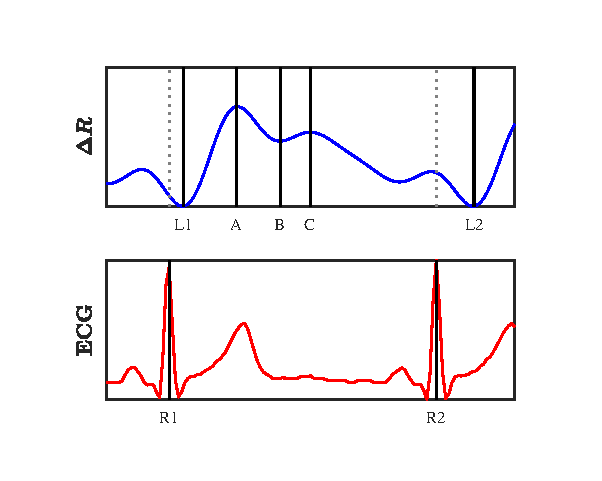
\includegraphics[width=10cm,keepaspectratio]{figure_apa_1}
	\caption[Marker ppoints in an iPG waveform]{Peaks and valleys of an iPG waveform ($\Delta R$) compared to ECG waveform.}
	\label{fig:markers iPG}
\end{figure}

Commonly, an APA wave consists of several identifiable peaks and valleys. Figure \ref{fig:markers iPG} shows a typical impedance plethysmography pulse synchronous with a heartbeat along with a limb. The table \ref{tbl:APA markers} summarises the noticeable markers of the pulse waveforms when compared with an ECG.

\begin{table}[!htpb]
	\caption{Markers on the APA waveform}
	\label{tbl:APA markers}
	\centering
	\begin{tabular}{c p{10cm}}
		\textbf{Marker} & \textbf{Description} \\
		\toprule
		R1 & Peak of the ECG QRS complex before an APA pulse. \\
		L1 & Start of the systolic upslope of the APA signal. Point where  rapid change of impedance occurs. \\
		A & Systolic point. Maximum peak of the APA signal.  \\
		B & Dicrotic notch on the APA wave. \\
		C & Maximum pulse after the dicrotic notch, named diastolic pulse  \\
		R2 & Peak of the ECG QRS complex after the APA pulse.  \\
		L2 & Starting point of the next APA wave. \\
		\bottomrule
	\end{tabular}
\end{table}

An APA wave has to be identified as a valid one to be included in the computational analysis. Therefore, the programmed algorithm starts through the identification of the beginning and the end of a pulse by locating the upslope point $L1$ and $L2$ in the waveform. Once this spot has been identified, the systolic peak $A$ can be placed. Follow, the point $B$ is expected to be a valley with an amplitude below the previous peak. Then, the algorithm looks the following change of slope which is the diastolic peak $C$. In case that any of these conditions were not met, then the algorithm searches the APA wave from the next lower data point, looking for a matching wave pattern again. If a pattern is found ($L1 > A < B > slope change (C) > L2$), then this is count as a fixed wave. If there not match the pulse is marked as missing. Also, to minimise waves with abnormal amplitudes caused by noise, the algorithm calculates the mean peak at $A$ of the last 20 valid APA waves. If the value is greater than \SI{25}{\percent} ($A > A*1.25$) then the wave is discarded.

The table \ref{tbl:detect APA} compiles the amount of APA waves recognised by the algorithm. The column \textit{detected waves} describes the pulses that comply with the profile of an iPG plethysmography wave. The third column shows the pulses that did not match the expected guide; then the algorithm tried to fix them by identifying the pattern in the next slope. As a result, the fixed column shows the total of pulse identified and the last column the ones discarded.

In general, the quality of the APA pulses validated by the iPG device and verified by the algorithm were in average \SI{57.86(1637)}{\percent}. Participants 3, 4 and 8 displayed the highest number of pulses with errors (above \SI{50}{\percent}). However, by performing the fixing method the amount valid peaks improved to a total of \SI{84.94(764)}{\percent}.

\begin{table}[!htbp]
	\caption{Change of amplitude of the waveform at peak A during the transition from baseline to venous occlusion.}
	\label{tbl:detect APA}
	\centering\small
	\begin{tabular}{lrrr>{\columncolor[gray]{0.8}}l>{\columncolor[gray]{0.9}}l}
		\toprule
		& \multicolumn{1}{c}{\textbf{Total}}
		& \multicolumn{1}{c}{\textbf{Detected}} & \multicolumn{1}{c}{\textbf{Waves}}& \multicolumn{1}{c}{\textbf{Fixed}} & \multicolumn{1}{c}{\textbf{Discarded}} \\
		& \multicolumn{1}{c}{\textbf{valleys}} & \multicolumn{1}{c}{\textbf{waves}} & \multicolumn{1}{c}{\textbf{with errors}}& \multicolumn{1}{c}{\textbf{waves}} & \multicolumn{1}{c}{\textbf{waves}} \\
		\midrule
		Participant 1	&1604	& 840 (\SI{52.37}{\percent})	&764 (\SI{47.63}{\percent})	&491 (\SI{30.61}{\percent})	&273 (\SI{17.02}{\percent})\\
		Participant 2	&1689	&1159 (\SI{68.62}{\percent})	&530 (\SI{31.38}{\percent})	&409 (\SI{24.22}{\percent})	&121 ( \SI{7.16}{\percent})\\
		Participant 3	&1651	& 699 (\SI{42.34}{\percent})	&952 (\SI{57.66}{\percent})	&695 (\SI{42.10}{\percent})	&257 (\SI{15.57}{\percent})\\
		Participant 4	&1625	& 645 (\SI{39.69}{\percent})	&980 (\SI{60.31}{\percent})	&562 (\SI{34.58}{\percent})	&418 (\SI{25.72}{\percent})\\
		Participant 5	&1664	&1199 (\SI{72.06}{\percent})	&465 (\SI{27.94}{\percent})	&345 (\SI{20.73}{\percent})	&120 ( \SI{7.21}{\percent})\\
		Participant 6	&1745	& 936 (\SI{53.64}{\percent})	&809 (\SI{46.36}{\percent})	&471 (\SI{26.99}{\percent})	&338 (\SI{19.37}{\percent})\\
		Participant 7	&1907	&1654 (\SI{86.73}{\percent})	&253 (\SI{13.27}{\percent})	&146 ( \SI{7.66}{\percent})	&107 ( \SI{5.61}{\percent})\\
		Participant 8	&1651	& 784 (\SI{47.49}{\percent})	&867 (\SI{52.51}{\percent})	&491 (\SI{29.74}{\percent})	&376 (\SI{22.77}{\percent})\\
		\bottomrule
	\end{tabular}
\end{table}

From these data, the changes during each occlusion among the points $A$, $B$ and $C$  were examined. The following analysis centres in the changes of impedance amplitude all along the different regions of the experiment, and the change of area of the waveform before and after the dicrotic notch point ($B$).


%%********************************** % Section 8.2 ******************************************
\section{Changes of the plethysmography waveform during different occlusions}
\label{section apa 2}
From the detection of the APA waveforms are possible to analyse the change of the shape form independently. For this, an average waveform was computed for each of the regions during the experiment. The following section details the changes for each of the points of interest. 

%%********************************** % Section 8.2.1 ******************************************
\subsection{Plethysmography waveform change during venous occlusion}
\label{section apa 2.1}
The analysis performed in this section corresponds to the APA waveforms captured during baseline in region 1 (\SIrange{0}{300}{\second}), venous occlusion (\SIrange{300}{480}{\second}) and return to control signal (\SIrange{480}{780}{\second}).  The previous section described the method how the valid pulses were collected. Consequently, all the valid pulses were grouped and aligned per region calculating the average waveform.


%This method allows multifigures being aligned using subcaptionbox
\begin{figure*}[!htbp]
	\centering
	\null\hfill%
	\subcaptionbox{Average APA waveform for baseline region 1 (\SIrange{0}{300}{\second})\label{fig:iPG_venous_baseline}}
	[0.48\textwidth]{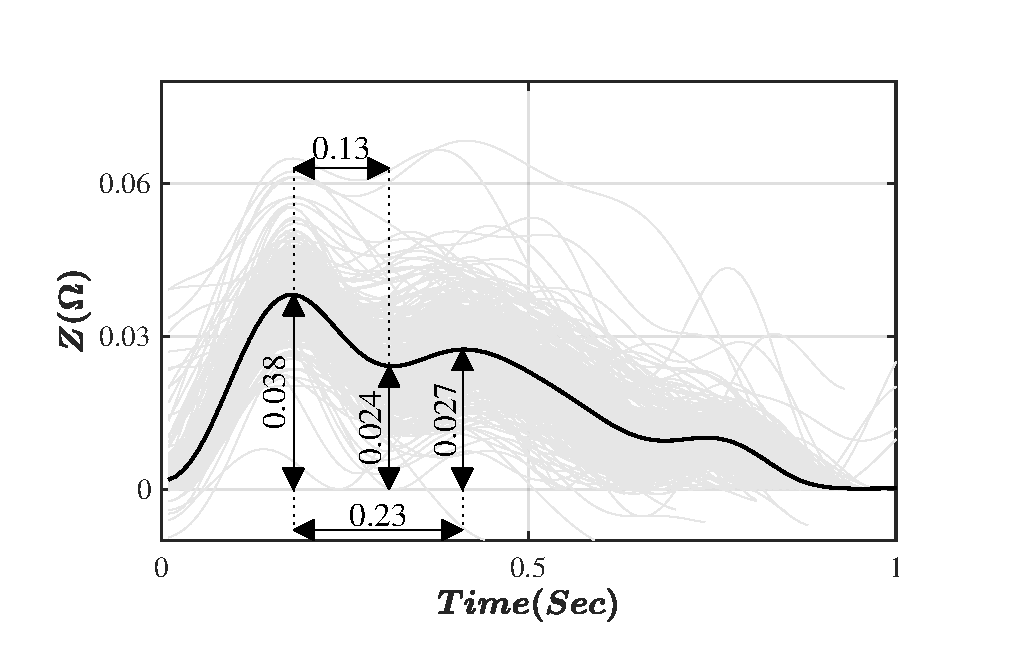
\includegraphics[width=0.48\textwidth, trim={0.5cm 0cm 1.5cm 0 cm}, clip]{figure_apa_2a}}%
	\hfill%
	\subcaptionbox{Average APA waveform during venous occlusion region 2 (\SIrange{300}{480}{\second})\label{fig:iPG_venous_occlusion}}
	[0.48\textwidth]{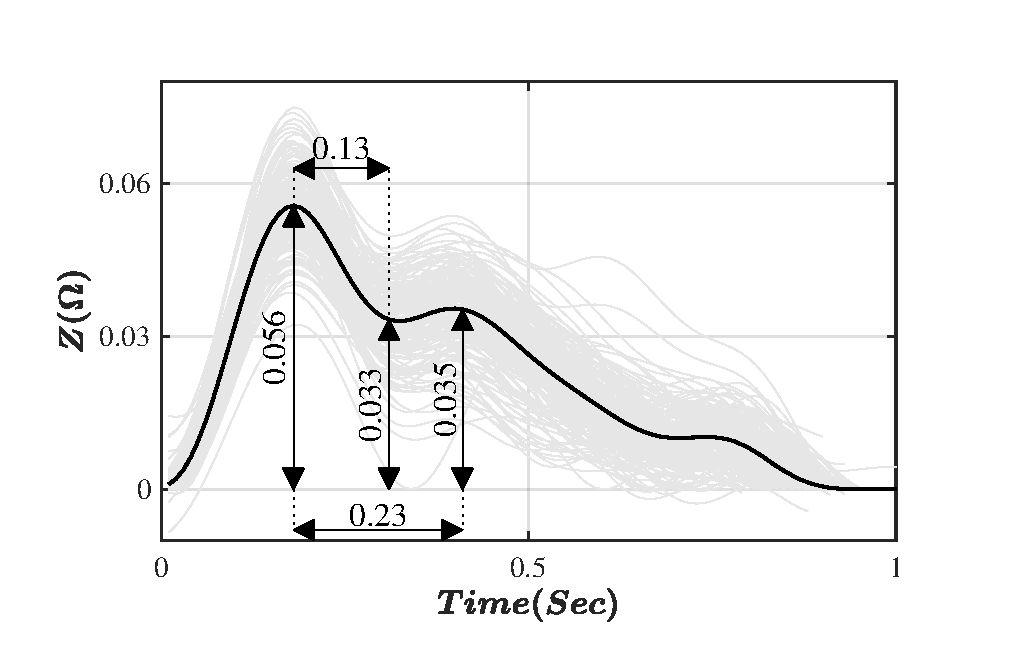
\includegraphics[width=0.48\textwidth, trim={0.5cm 0cm 1.5cm 0 cm}, clip]{figure_apa_2b}}%
	\hfill\null%
	\caption{Plethysmography waveform of the participant seven between baseline and venous occlusion}
	\label{fig:iPG_venous}
	
	\vspace{1cm}
	
	\null\hfill%
	\subcaptionbox{Change of amplitude of the waveform at point A.\label{fig:change A venous}}
	[0.48\textwidth]{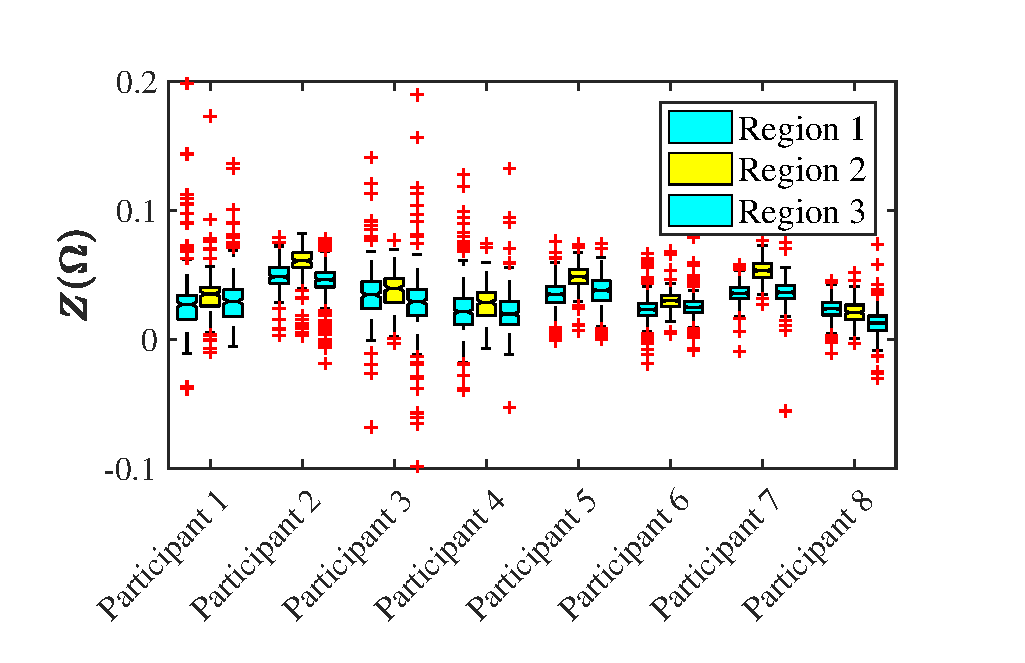
\includegraphics[width=0.48\textwidth, trim={0.5cm 0cm 1.5cm 0 cm}, clip]{figure_apa_3a}}%
	\hfill%
	\subcaptionbox{Change of amplitude of the waveform at point B.\label{fig:change B venous}}
	[0.48\textwidth]{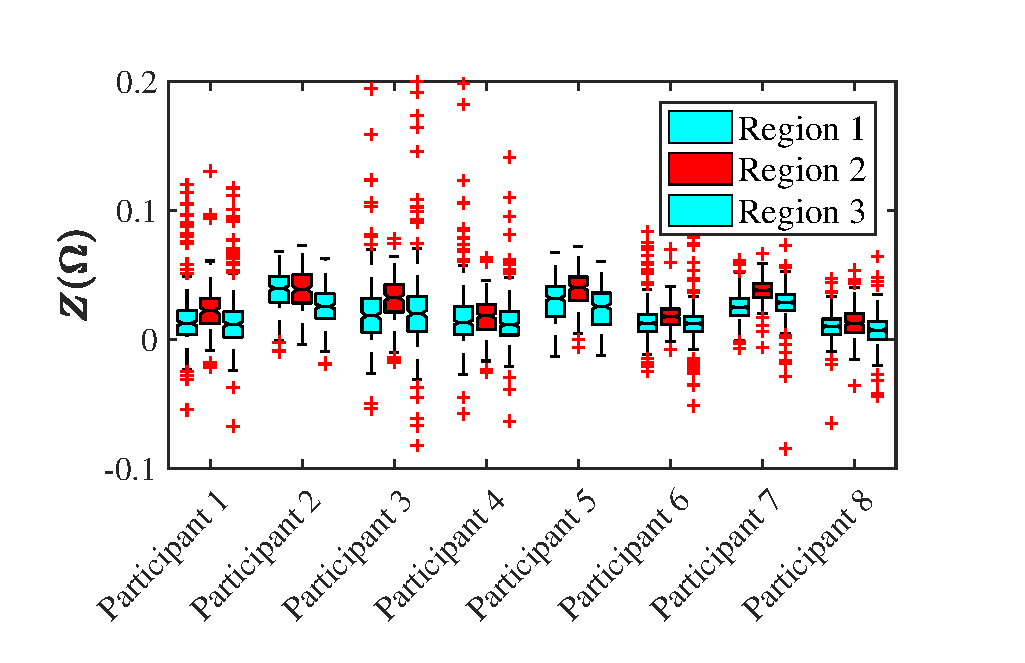
\includegraphics[width=0.48\textwidth, trim={0.5cm 0cm 1.5cm 0 cm}, clip]{figure_apa_3b}}%
	\hfill%
	\subcaptionbox{Change of amplitude of the waveform at point C.\label{fig:change C venous}}
	[0.48\textwidth]{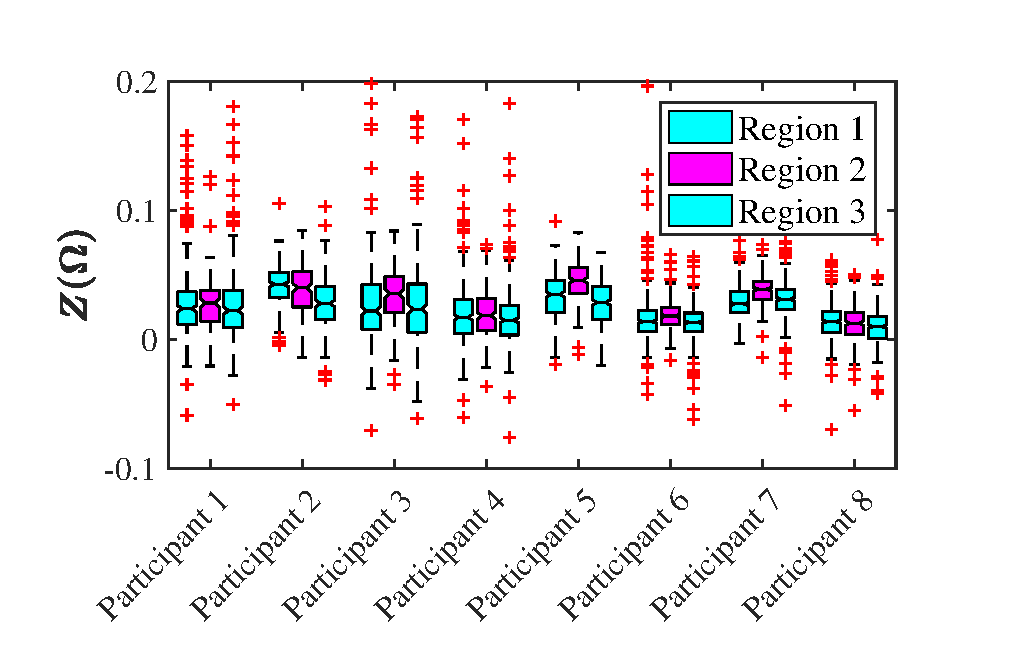
\includegraphics[width=0.48\textwidth, trim={0.5cm 0cm 1.5cm 0 cm}, clip]{figure_apa_3c}}%
	\null%
	\caption{Changes of the impedance peak values during baseline, venous occlusion and return to baseline for points A,B and C.}
	\label{fig:iPG change points venous}
\end{figure*}

Figure \ref{fig:iPG_venous_baseline} shows an impedance plethysmography waveform calculated from one of the participants during baseline and venous occlusion, with indicators of their amplitudes at the different points of interest. Some of the markers show the calculation of the distance between systolic peak (Point A) to dicrotic notch (Point B) and diastolic peak (Point C), as well as, the amplitude for each of these markers. The distance between (A $\rightarrow$ B) and (A $\rightarrow$ C) was later transposed into the occlusion wave to identify their values during the VOP test.


Clearly,  from a qualitative point of view, one can notice that there is a difference in the morphology of the waveform during the occlusion.  Indeed, figure \ref{fig:iPG change points venous} shows the change of the amplitude at these points for every participant and the return to baseline after the cuff pressure was released. A complete analysis of the change at each point is detailed as follows.


\subsubsection{Changes in systolic peak (Point A)}
\label{section apa 2.1.1}
Figure \ref{fig:change A venous} shows the statistical variation of the systolic peak magnitude (point A) during the three conditions of the test baseline-occlusion-baseline. After inflating the cuff below the diastolic pressure, most of the APA signals displayed an increase of the impedance magnitude of this peak. Indeed, as detailed in table \ref{tbl:change A venous}, \SI{87}{\percent} of the participants showed an increment in electrical resistance during venous occlusion of about \SI{31.80}{\percent}, only participant 8 was an exception where his/her impedance decreased in \SI{-12.01}{\percent}. Then, when the cuff's pressure was released, all the participants showed a decline of the peak value with an average of \SI{-32.21}{\percent}, returning to similar baseline values before the venous occlusion.

\begin{table}[!htbp]
	\caption[Change of amplitude of the waveform at peak A during the transition baseline-venous occlusion-baseline.]{Change of amplitude of the waveform at peak A during the transition from baseline (region 1), venous occlusion (region 2) and return to baseline (region 3). The column change shows the percentile variations between the different regions.}
	\label{tbl:change A venous}
	\centering\small
\begin{tabular}{l
				*{3}{S[table-format=1.4]@{\,\( \pm \)\,}S[table-format=1.4]} %Format for Z+-std
		       >{\columncolor[gray]{0.8}}c>{\columncolor[gray]{0.9}}c}
	\toprule
	& \multicolumn{2}{c}{\multirow{2}{*}{\textbf{Baseline [\si{\ohm}]}}}
	& \multicolumn{2}{c}{\multirow{2}{*}{\textbf{Occlusion [\si{\ohm}]}}}
	& \multicolumn{2}{c}{\multirow{2}{*}{\textbf{Baseline [\si{\ohm}]}}}
	& \multicolumn{2}{c}{\textbf{Change}} \\
	& \multicolumn{2}{c}{}
	& \multicolumn{2}{c}{}
	& \multicolumn{2}{c}{}
	&\textbf{R1-R2}&\textbf{R2-R3}\\\midrule
    Participant 1 & 0.0270 & 0.0233 & 0.0353 & 0.0191 & 0.0295 & 0.0305 & 30.49 \% & -21.41 \% \\
	Participant 2 & 0.0485 & 0.0102 & 0.0609 & 0.0140 & 0.0462 & 0.0449 & 25.50 \% & -30.24 \% \\
	Participant 3 & 0.0345 & 0.0351 & 0.0397 & 0.0144 & 0.0292 & 0.0294 & 14.96 \% & -30.55 \% \\
	Participant 4 & 0.0214 & 0.0303 & 0.0289 & 0.0139 & 0.0197 & 0.0222 & 35.17 \% & -43.11 \% \\
	Participant 5 & 0.0352 & 0.0112 & 0.0485 & 0.0098 & 0.0382 & 0.0376 & 37.99 \% & -29.20 \% \\
	Participant 6 & 0.0232 & 0.0105 & 0.0300 & 0.0124 & 0.0249 & 0.0251 & 29.16 \% & -21.77 \% \\
	Participant 7 & 0.0357 & 0.0080 & 0.0534 & 0.0081 & 0.0365 & 0.0365 & 49.33 \% & -47.17 \% \\
	Participant 8 & 0.0238 & 0.0094 & 0.0209 & 0.0091 & 0.0128 & 0.0127 &-12.01 \% & -34.27 \% \\ \bottomrule
\end{tabular}
\end{table}


\subsubsection{Changes in dicrotic notch peak (Point B)}
\label{section apa 2.1.2}
The dicrotic notch (point B) is located between the systolic (point A) and diastolic peaks (point C) as represented in figure \ref{fig:markers iPG}.  Similarly, as the changes experienced by the systolic peak during this part of the experiment, the point B also increased in its magnitude. After that, when the cuff's pressure was released the amplitude at this location returned to an amplitude quite close to the baseline.

According to the data shown on Table \ref{tbl:change B venous}, one can see that most of the participants (\SI{87.5}{\percent}) showed an increase in the magnitude of their dicrotic notch point. Certainly, between those who experienced this increment, the impedance changed roughly \SI{47.73}{\percent} compared to the measurement at region 1. However, partaker two noted a slight decrease in their measured impedance \SI{-2.06}{\percent} which was not very significant compared to the others. In contrast, after releasing the upper arms blockage, all the participants experienced a drop of their point B magnitude of about  \SI{-51.68}{\percent}.

\begin{table}[!htbp]
	\caption{Change of amplitude of the waveform at peak B during the transition from baseline to venous occlusion.}
	\label{tbl:change B venous}
	\centering\small
	\begin{tabular}{l
					*{3}{S[table-format=1.4]@{\,\( \pm \)\,}S[table-format=1.4]} %Format for Z+-std
					>{\columncolor[gray]{0.8}}c>{\columncolor[gray]{0.9}}c}
	\toprule
	& \multicolumn{2}{c}{\multirow{2}{*}{\textbf{Baseline [\si{\ohm}]}}}
	& \multicolumn{2}{c}{\multirow{2}{*}{\textbf{Occlusion [\si{\ohm}]}}}
	& \multicolumn{2}{c}{\multirow{2}{*}{\textbf{Baseline [\si{\ohm}]}}}
	& \multicolumn{2}{c}{\textbf{Change}} \\
	& \multicolumn{2}{c}{}
	& \multicolumn{2}{c}{}
	& \multicolumn{2}{c}{}
	&\textbf{R1-R2}&\textbf{R2-R3}\\\midrule
	Participant 1 & 0.0126 & 0.0231 & 0.0223 & 0.0195 & 0.0119 & 0.0153 & 76.94 \% & -82.52 \% \\
	Participant 2 & 0.0397 & 0.0144 & 0.0388 & 0.0167 & 0.0257 & 0.0252 & -2.06 \% & -33.19 \% \\
	Participant 3 & 0.0184 & 0.0315 & 0.0323 & 0.0181 & 0.0200 & 0.0224 & 75.98 \% & -67.36 \% \\
	Participant 4 & 0.0130 & 0.0294 & 0.0183 & 0.0149 & 0.0113 & 0.0138 & 40.21 \% & -53.52 \% \\
	Participant 5 & 0.0319 & 0.0158 & 0.0402 & 0.0138 & 0.0254 & 0.0237 & 25.92 \% & -46.26 \% \\
	Participant 6 & 0.0127 & 0.0138 & 0.0177 & 0.0161 & 0.0124 & 0.0128 & 39.75 \% & -41.55 \% \\
	Participant 7 & 0.0250 & 0.0108 & 0.0382 & 0.0092 & 0.0287 & 0.0276 & 52.71 \% & -37.97 \% \\
	Participant 8 & 0.0102 & 0.0111 & 0.0125 & 0.0117 & 0.0073 & 0.0071 & 22.58 \% & -51.08 \% \\
 \bottomrule
	\end{tabular}
\end{table}

\subsubsection{Changes in diastolic peak (Point C)}
\label{section apa 2.1.3}
The last peak analysed corresponds to the point C or diastolic peak of the waveform. Again, figure \ref{fig:change C venous} shows that most of the participants (\SI{71.4}{\percent}) showed an increase in the magnitude at this point of about \SI{31.92}{\percent} compared to region 1. Only, participants 2 and 8 described a slight decrease of their impedance in an average of \SI{-7.97}{\percent}. Table \ref{tbl:change C venous} shows the mean values of the impedance at this location in the waveform. In contrast, after releasing the upper arm's pressure, all the participants experienced a decrease in their diastolic peak impedance, with an average of \SI{-32.33}{\percent}. Hence, the diastolic peak returned to values similar to the baseline, except for the ones that experience a decrease in resistance during the occlusion.

\begin{table}[!htbp]
	\caption{Change of amplitude of the waveform at peak C during the transition from baseline to venous occlusion.}
	\label{tbl:change C venous}
	\centering\small
	\begin{tabular}{l
					*{3}{S[table-format=1.4]@{\,\( \pm \)\,}S[table-format=1.4]} %Format for Z+-std
					>{\columncolor[gray]{0.8}}c>{\columncolor[gray]{0.9}}c}
	\toprule
	& \multicolumn{2}{c}{\multirow{2}{*}{\textbf{Baseline [\si{\ohm}]}}}
	& \multicolumn{2}{c}{\multirow{2}{*}{\textbf{Occlusion [\si{\ohm}]}}}
	& \multicolumn{2}{c}{\multirow{2}{*}{\textbf{Baseline [\si{\ohm}]}}}
	& \multicolumn{2}{c}{\textbf{Change}} \\
	& \multicolumn{2}{c}{}
	& \multicolumn{2}{c}{}
	& \multicolumn{2}{c}{}
	&\textbf{R1-R2}&\textbf{R2-R3}\\\midrule
    Participant 1 & 0.0238 & 0.0281 & 0.0283 & 0.0260 & 0.0224 & 0.0286 & 18.81 \% & -24.75 \% \\
	Participant 2 & 0.0429 & 0.0150 & 0.0401 & 0.0191 & 0.0279 & 0.0278 & -6.48 \% & -28.45 \% \\
	Participant 3 & 0.0221 & 0.0397 & 0.0355 & 0.0219 & 0.0236 & 0.0310 & 60.85 \% & -53.94 \% \\
	Participant 4 & 0.0171 & 0.0380 & 0.0184 & 0.0174 & 0.0149 & 0.0178 &  7.42 \% & -20.30 \% \\
	Participant 5 & 0.0350 & 0.0175 & 0.0459 & 0.0151 & 0.0287 & 0.0279 & 31.16 \% & -49.18 \% \\
	Participant 6 & 0.0138 & 0.0212 & 0.0182 & 0.0251 & 0.0133 & 0.0151 & 31.53 \% & -35.22 \% \\
	Participant 7 & 0.0276 & 0.0127 & 0.0391 & 0.0111 & 0.0312 & 0.0309 & 41.77 \% & -28.58 \% \\
	Participant 8 & 0.0138 & 0.0140 & 0.0125 & 0.0163 & 0.0100 & 0.0096 & -9.47 \% & -18.24 \% \\

	\bottomrule
	\end{tabular}
\end{table}

%%********************************** % Section 8.2.2 ******************************************
\subsection{Plethysmography waveform change during partial arterial occlusion}
\label{section apa 2.2}
During the partial occlusion of the brachial artery, similarly to venous occlusion, most of the participants also showed a change in the shape of their waveforms. The analysis of this section resembles the baseline time in region 3 (\SIrange{480}{780}{\second}), three minutes of partial venous occlusion in region 4 (\SIrange{780}{960}{\second}) and return to baseline region 5 (\SIrange{960}{1260}{\second}). The cuff was inflated to the pressure presented in column \textit{Occlusion 2} in Table \ref{tbl:occlusions}, laying between diastolic ans systolic pressures.

Figure \ref{fig:iPG arterial} shows the average waveform of all the signals aligned at baseline and during the arm's occlusion for one of the participants. As is evident from the plot, there is an increase in the systolic peak (point A) and a reduction in the diastolic peak at point C). Figure \ref{fig:iPG change points arterial} also features the impedance change in each participant during the three regions of the experiment. The following sections will describe in detail the changes to each of the spots.

%This method allows multifigures being aligned using subcaptionbox
\begin{figure*}
	\centering
	\null\hfill%
	\subcaptionbox{Average plethysmography waveform during venous occlusion region 3 (\SIrange{480}{780}{\second})\label{fig:iPG arterial baseline}}
	[0.48\textwidth]{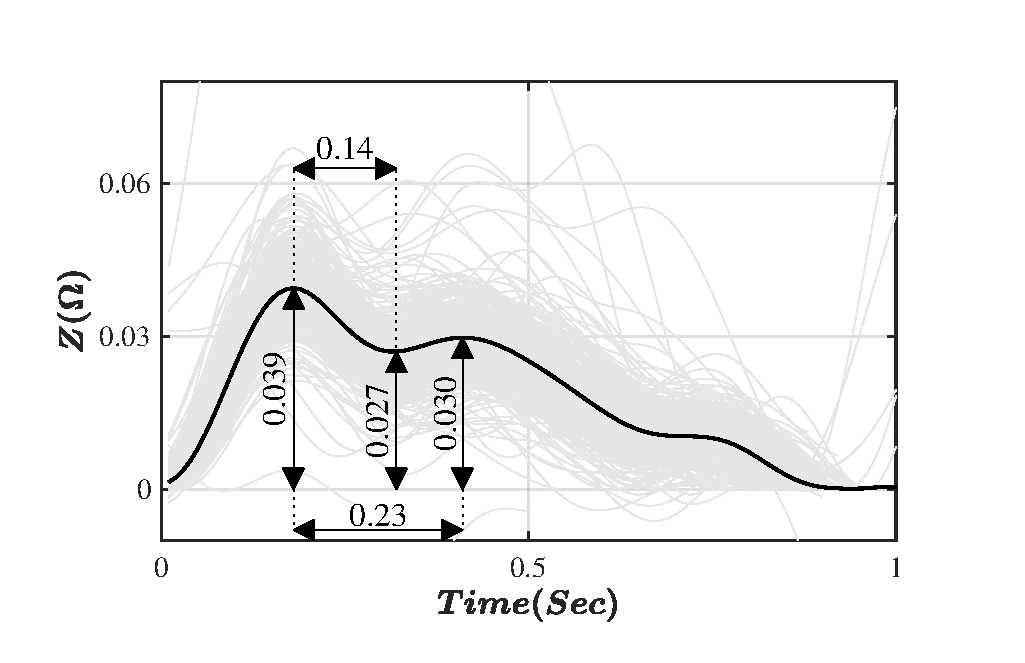
\includegraphics[width=0.48\textwidth, trim={0.5cm 0cm 1.5cm 0 cm}, clip]{figure_apa_4a}}%
	\hfill%
	\subcaptionbox{Average plethysmography waveform during venous occlusion region 4 (\SIrange{780}{960}{\second})\label{fig:iPG arterial occlusion}}
	[0.48\textwidth]{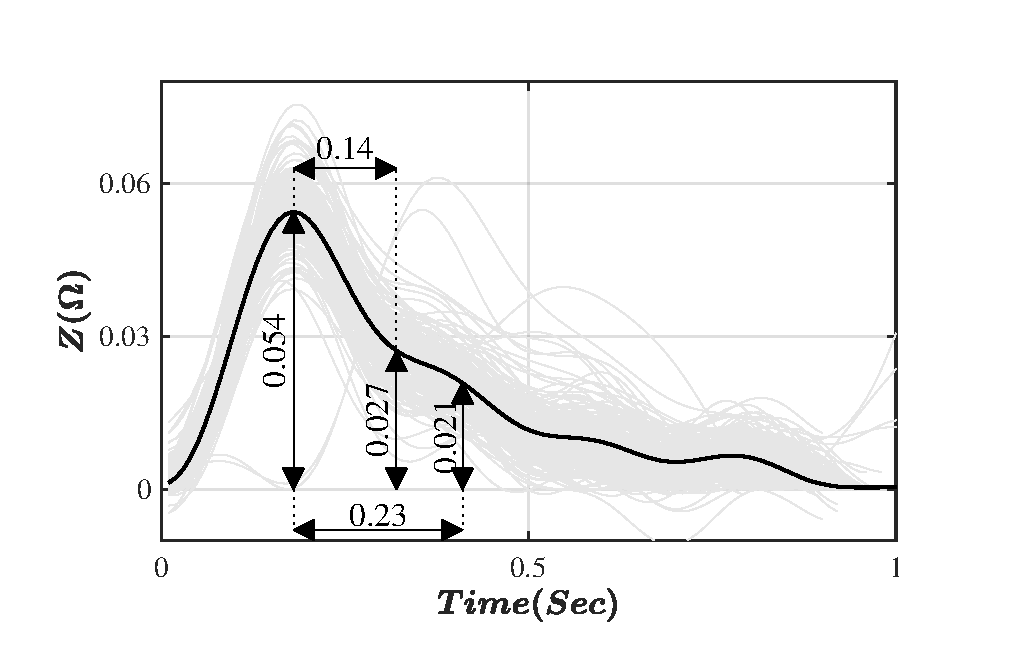
\includegraphics[width=0.48\textwidth, trim={0.5cm 0cm 1.5cm 0 cm}, clip]{figure_apa_4b}}%
	\hfill\null%
	\caption{Plethysmography waveform of the participant seven between baseline and partial arterial occlusion}
	\label{fig:iPG arterial}

	\vspace{1cm}

	\null\hfill%
	\subcaptionbox{Change of amplitude of the waveform at point A.\label{fig:change A arterial}}
	[0.48\textwidth]{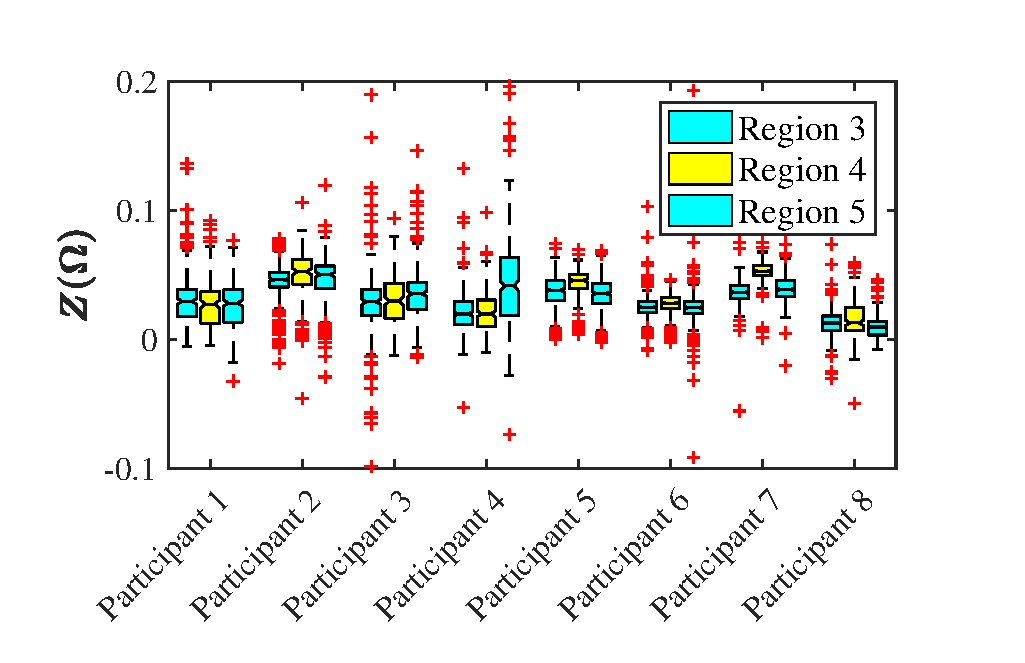
\includegraphics[width=0.48\textwidth, trim={0.5cm 0cm 1.5cm 0 cm}, clip]{figure_apa_5a}}%
	\hfill%
	\subcaptionbox{Change of amplitude of the waveform at point B.\label{fig:change B arterial}}
	[0.48\textwidth]{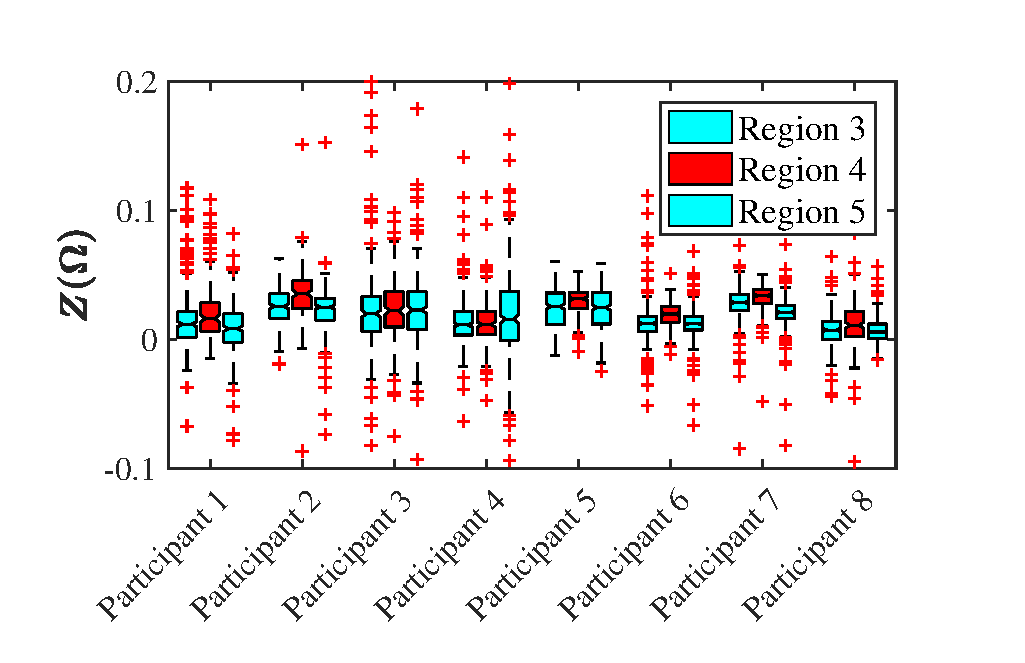
\includegraphics[width=0.48\textwidth, trim={0.5cm 0cm 1.5cm 0 cm}, clip]{figure_apa_5b}}%
	\hfill%
	\subcaptionbox{Change of amplitude of the waveform at point C.\label{fig:change C arterial}}
	[0.48\textwidth]{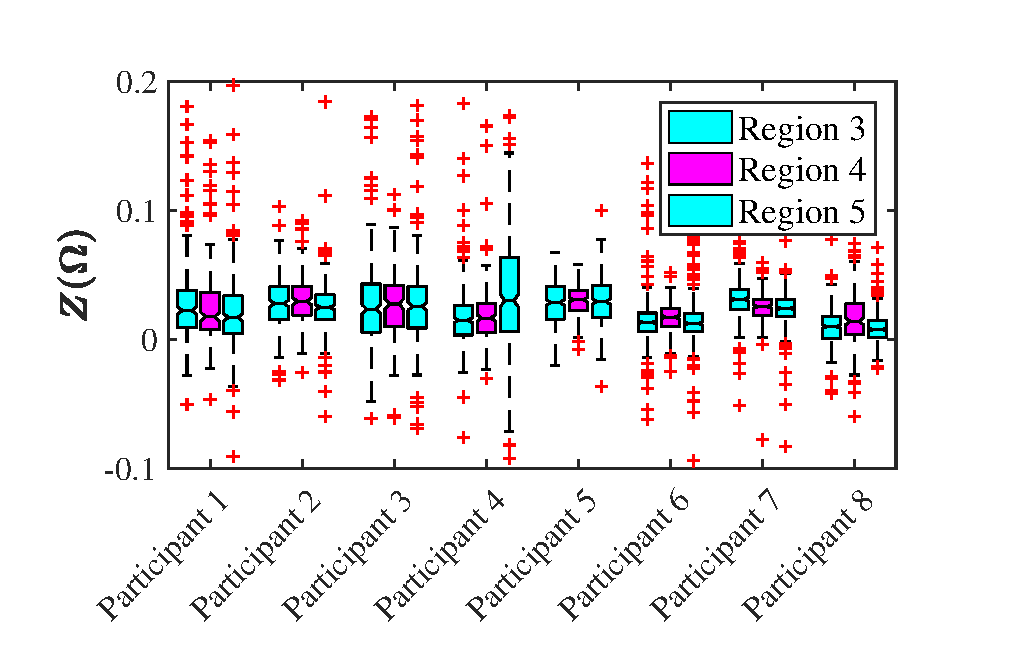
\includegraphics[width=0.48\textwidth, trim={0.5cm 0cm 1.5cm 0 cm}, clip]{figure_apa_5c}}%
	\null%
	\caption{Changes of the impedance peak values during baseline, partial arterial occlusion and return to baseline for points A,B and C.}
	\label{fig:iPG change points arterial}
\end{figure*}

\subsubsection{Changes in systolic peak (Point A)}
\label{section apa 2.2.1}
Figure \ref{fig:change A arterial} indicates the change in amplitude for each one of the participants. Also, table \ref{tbl:change A arterial} summarises the average impedances and the variations in each region. Through this occlusive experiment, 7 participants (\SI{87.5}{\percent}) displayed an increase in electrical resistivity at point A of about \SI{13.52}{\percent}. However, some of these participants showed a tiny increase in their peaks between \SIrange{0.29}{2.24}{\percent}. In general, one can note the hike at this point. After the cuff was deflated, most of the participants (\SI{62.5}{\percent}) showed a decrease of the peak in an average of \SI{-21.86}{\percent}.  In contrast, participants one, three and four registered an increase in their impedance reading, being the later an outlier with an increase in his magnitude of \SI{110.69}{\percent}.

\begin{table}[!htbp]
	\caption{Change of amplitude of the waveform at peak A during the transition from baseline to venous occlusion.}
	\label{tbl:change A arterial}
	\centering\small
	\begin{tabular}{l
					*{3}{S[table-format=1.4]@{\,\( \pm \)\,}S[table-format=1.4]} %Format for Z+-std
					>{\columncolor[gray]{0.8}}c>{\columncolor[gray]{0.9}}c}
		\toprule
		& \multicolumn{2}{c}{\multirow{2}{*}{\textbf{Baseline [\si{\ohm}]}}}
		& \multicolumn{2}{c}{\multirow{2}{*}{\textbf{Occlusion [\si{\ohm}]}}}
		& \multicolumn{2}{c}{\multirow{2}{*}{\textbf{Baseline [\si{\ohm}]}}}
		& \multicolumn{2}{c}{\textbf{Change}} \\
		& \multicolumn{2}{c}{}
		& \multicolumn{2}{c}{}
		& \multicolumn{2}{c}{}
		&\textbf{R3-R4}&\textbf{R4-R5}\\\midrule
	    Participant 1 & 0.0295 & 0.0194 & 0.0274 & 0.0190 & 0.0282 & 0.0265 & -7.03 \% &   2.59 \% \\
		Participant 2 & 0.0462 & 0.0140 & 0.0526 & 0.0197 & 0.0503 & 0.0461 & 13.78 \% &  -5.11 \% \\
		Participant 3 & 0.0292 & 0.0379 & 0.0298 & 0.0185 & 0.0354 & 0.0356 &  2.24 \% &  19.02 \% \\
		Participant 4 & 0.0197 & 0.0242 & 0.0198 & 0.0152 & 0.0416 & 0.0453 &  0.29 \% & 110.69 \% \\
		Participant 5 & 0.0382 & 0.0133 & 0.0458 & 0.0115 & 0.0357 & 0.0351 & 19.81 \% & -26.55 \% \\
		Participant 6 & 0.0249 & 0.0096 & 0.0282 & 0.0081 & 0.0247 & 0.0251 & 13.21 \% & -14.09 \% \\
		Participant 7 & 0.0365 & 0.0097 & 0.0529 & 0.0092 & 0.0388 & 0.0394 & 44.90 \% & -38.73 \% \\
		Participant 8 & 0.0128 & 0.0104 & 0.0128 & 0.0160 & 0.0096 & 0.0098 &  0.38 \% & -24.86 \% \\
		\bottomrule
	\end{tabular}
\end{table}\subsubsection{Changes in dicrotic notch peak (Point B)}
\label{section apa 2.2.2}
In the dicrotic notch position (point B), the increase of its magnitude is clearer than in the systolic peak. In fact, all the participants depicted an increase in their impedance value at this point. Figure \ref{fig:change B arterial} evidence these shifts in each of the regions before and after the occlusion. Table \ref{fig:change B arterial} details participants' median impedances and the ratio of change in each region.

In general, the average increase at the dicrotic notch as soon as the occlusion was applied was about \SI{29.91}{\percent}. When the pressure restricting the blood flow was removed, six out of eight of the study members experienced a fall in electrical resistivity towards baseline. On average, it reduced by \SI{-51.72}{\percent}. Again, participant four was the exception to this reduction, as well as participant three. Their impedance rose by \SI{37.37}{\percent} and \SI{3.25}{\percent} respectively.

\begin{table}[!htbp]
	\caption{Change of amplitude of the waveform at peak B during the transition from baseline to venous occlusion.}
	\label{tbl:change B arterial}
	\centering\small
	\begin{tabular}{l
					*{3}{S[table-format=1.4]@{\,\( \pm \)\,}S[table-format=1.4]} %Format for Z+-std
					>{\columncolor[gray]{0.8}}c>{\columncolor[gray]{0.9}}c}
		\toprule
		& \multicolumn{2}{c}{\multirow{2}{*}{\textbf{Baseline [\si{\ohm}]}}}
		& \multicolumn{2}{c}{\multirow{2}{*}{\textbf{Occlusion [\si{\ohm}]}}}
		& \multicolumn{2}{c}{\multirow{2}{*}{\textbf{Baseline [\si{\ohm}]}}}
		& \multicolumn{2}{c}{\textbf{Change}} \\
		& \multicolumn{2}{c}{}
		& \multicolumn{2}{c}{}
		& \multicolumn{2}{c}{}
		&\textbf{R3-R4}&\textbf{R4-R5}\\\midrule
		Participant 1 & 0.0119 & 0.0232 & 0.0162 & 0.0220 & 0.0083 & 0.0087 & 36.07 \% & -66.02 \% \\
		Participant 2 & 0.0257 & 0.0142 & 0.0354 & 0.0212 & 0.0251 & 0.0231 & 38.02 \% & -40.44 \% \\
		Participant 3 & 0.0200 & 0.0536 & 0.0222 & 0.0247 & 0.0229 & 0.0244 & 11.33 \% &   3.25 \% \\
		Participant 4 & 0.0113 & 0.0256 & 0.0116 & 0.0177 & 0.0158 & 0.0143 &  2.64 \% &  37.37 \% \\
		Participant 5 & 0.0254 & 0.0155 & 0.0314 & 0.0107 & 0.0248 & 0.0237 & 23.55 \% & -26.29 \% \\
		Participant 6 & 0.0124 & 0.0150 & 0.0197 & 0.0096 & 0.0121 & 0.0141 & 58.95 \% & -61.59 \% \\
		Participant 7 & 0.0287 & 0.0128 & 0.0340 & 0.0104 & 0.0211 & 0.0205 & 18.34 \% & -44.99 \% \\
		Participant 8 & 0.0073 & 0.0118 & 0.0110 & 0.0196 & 0.0058 & 0.0069 & 50.41 \% & -71.01 \% \\
\bottomrule
	\end{tabular}
\end{table}

\subsubsection{Changes in diastolic peak (Point C)}
\label{section apa 2.2.3}
Changes in the diastolic peak also presented a similar increasing trend as seen in points A and B. However; the changes were not as marked as the ones seen in the dicrotic notch. Figure \ref{fig:change C arterial} and Table \ref{tbl:change C arterial} summarise the values obtained. In total, \SI{75}{\percent} of the participants showed an increase of impedance between region 3 and 4. It increased with a median of \SI{18.74}{\percent}. Participant eight showed a change significantly larger than the mean (\SI{44.11}{\percent}). Study members one and seven pointed a decrease of electrical resistivity in \SI{-19.91}{\percent} on average.

On the opposite side of the exercise, after releasing the pressure, (\SI{87.5}{\percent}) of the partakers showed a reduction in their impedance, including those whose impedance rose during the occlusion. On average, impedance reduced by \SI{-19.77}{\percent} in total. Again, participant four showed an increase in the ratio of change before and after the blockage significantly exceeding the median of all the measurements. Moreover, this study member outperformed notably the average ratio after the occlusion (\SI{90.32}{\percent}). As portrayed by the other measuring points, this confirms that the data obtained from this study member were not from physiological origin but motion or randomness.

\begin{table}[!htbp]
	\caption{Change of amplitude of the waveform at peak C during the transition from baseline to venous occlusion.}
	\label{tbl:change C arterial}
	\centering\small
	\begin{tabular}{l
					*{3}{S[table-format=1.4]@{\,\( \pm \)\,}S[table-format=1.4]} %Format for Z+-std
					>{\columncolor[gray]{0.8}}c>{\columncolor[gray]{0.9}}c}
		\toprule
		& \multicolumn{2}{c}{\multirow{2}{*}{\textbf{Baseline [\si{\ohm}]}}}
		& \multicolumn{2}{c}{\multirow{2}{*}{\textbf{Occlusion [\si{\ohm}]}}}
		& \multicolumn{2}{c}{\multirow{2}{*}{\textbf{Baseline [\si{\ohm}]}}}
		& \multicolumn{2}{c}{\textbf{Change}} \\
		& \multicolumn{2}{c}{}
		& \multicolumn{2}{c}{}
		& \multicolumn{2}{c}{}
		&\textbf{R3-R4}&\textbf{R4-R5}\\\midrule
	    Participant 1 & 0.0224 & 0.0323 & 0.0176 & 0.0307 & 0.0171 & 0.0206 & -21.35 \% &  -2.21 \% \\
		Participant 2 & 0.0279 & 0.0196 & 0.0295 & 0.0272 & 0.0250 & 0.0252 &   5.96 \% & -16.45 \% \\
		Participant 3 & 0.0236 & 0.0826 & 0.0275 & 0.0284 & 0.0256 & 0.0283 &  16.56 \% &  -7.98 \% \\
		Participant 4 & 0.0149 & 0.0327 & 0.0166 & 0.0229 & 0.0301 & 0.0306 &  11.22 \% &  90.32 \% \\
		Participant 5 & 0.0287 & 0.0171 & 0.0308 & 0.0119 & 0.0293 & 0.0287 &   7.32 \% &  -5.03 \% \\
		Participant 6 & 0.0133 & 0.0252 & 0.0174 & 0.0111 & 0.0123 & 0.0176 &  30.32 \% & -37.72 \% \\
		Participant 7 & 0.0312 & 0.0189 & 0.0254 & 0.0124 & 0.0241 & 0.0232 & -18.48 \% &  -4.27 \% \\
		Participant 8 & 0.0100 & 0.0139 & 0.0141 & 0.0224 & 0.0076 & 0.0087 &  41.11 \% & -64.75 \% \\
		\bottomrule
	\end{tabular}
\end{table}

\subsection{Plethysmography waveform change during total occlusion}
\label{section apa 2.3}
%This method allows multifigures being aligned using subcaptionbox
\begin{figure*}
	\centering
	\null\hfill%
	\subcaptionbox{Average plethysmography waveform during venous occlusion region 5 (\SIrange{960}{1260}{\second})\label{fig:iPG_total_baseline}}
	[0.48\textwidth]{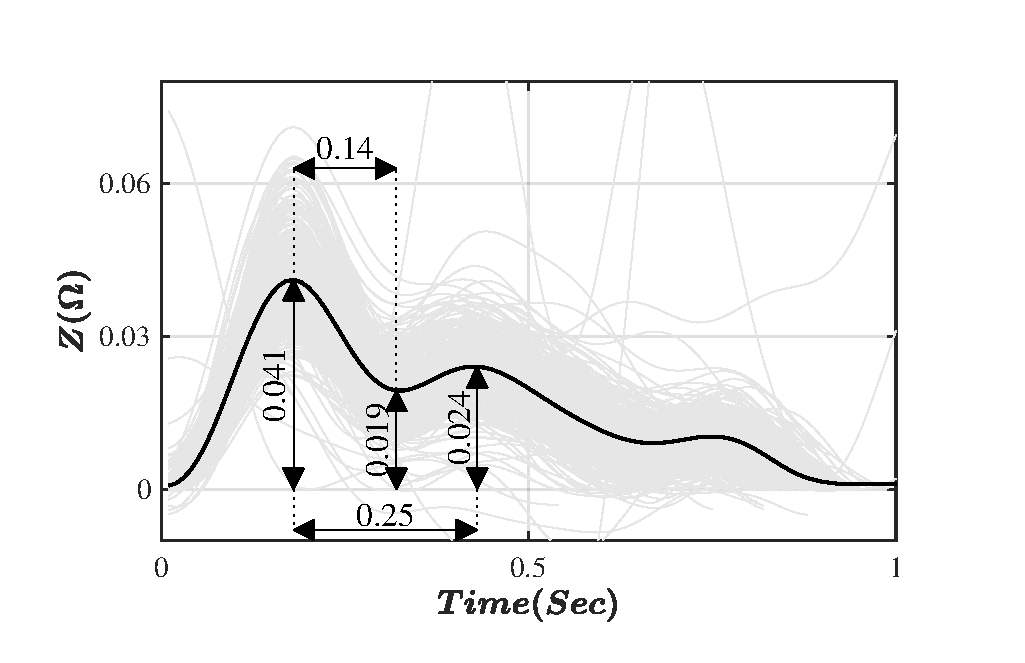
\includegraphics[width=0.48\textwidth, trim={0.5cm 0cm 1.5cm 0 cm}, clip]{figure_apa_6a}}%
	\hfill%
	\subcaptionbox{Average plethysmography waveform during venous occlusion region 6 (\SIrange{1260}{1440}{\second})\label{fig:iPG_total_occlusion}}
	[0.48\textwidth]{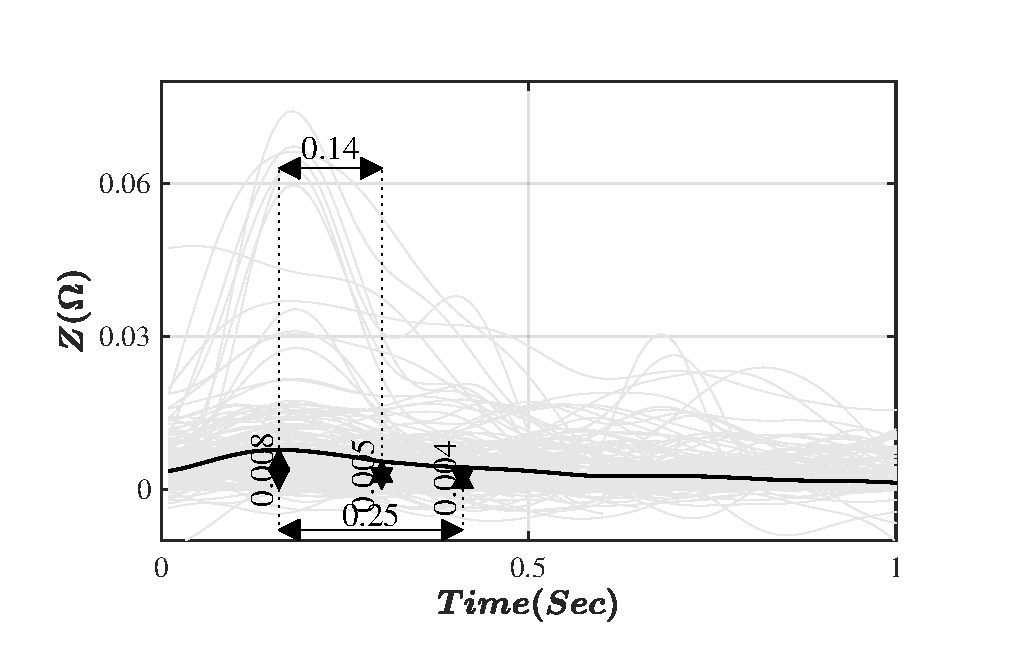
\includegraphics[width=0.48\textwidth, trim={0.5cm 0cm 1.5cm 0 cm}, clip]{figure_apa_6b}}%
	\hfill\null%
	\caption{Plethysmography waveform of the participant seven between baseline and total occlusion}
	\label{fig:iPG_total}
	
	\vspace{1cm}
	
	\null\hfill%
	\subcaptionbox{Change of amplitude of the waveform at point A.\label{fig:change_A_total}}
	[0.48\textwidth]{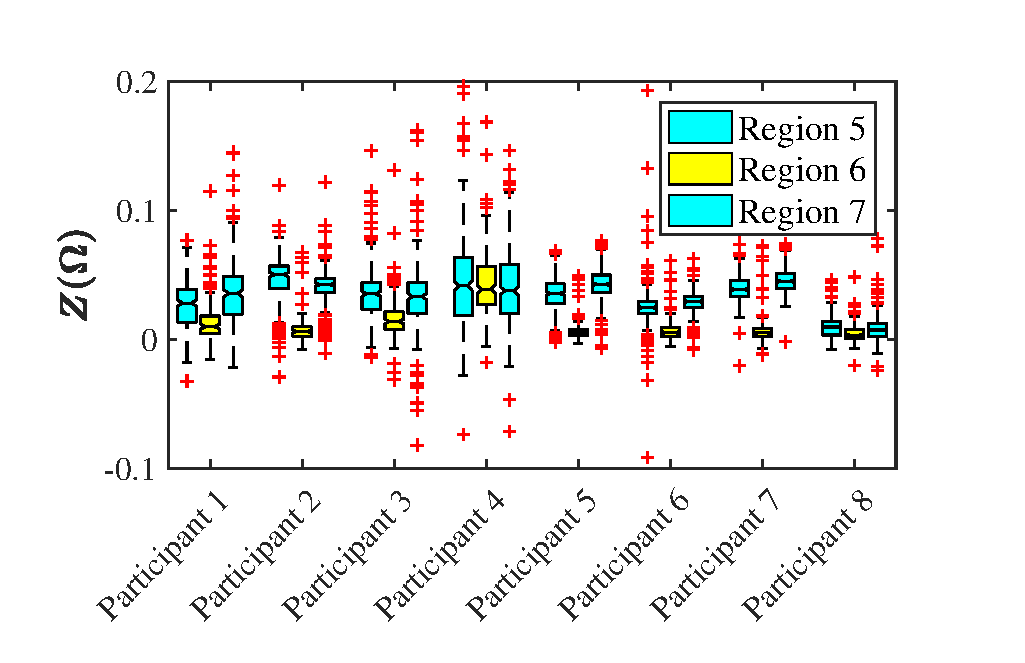
\includegraphics[width=0.48\textwidth, trim={0.5cm 0cm 1.5cm 0 cm}, clip]{figure_apa_7a}}%
	\hfill%
	\subcaptionbox{Change of amplitude of the waveform at point B.\label{fig:change_B_total}}
	[0.48\textwidth]{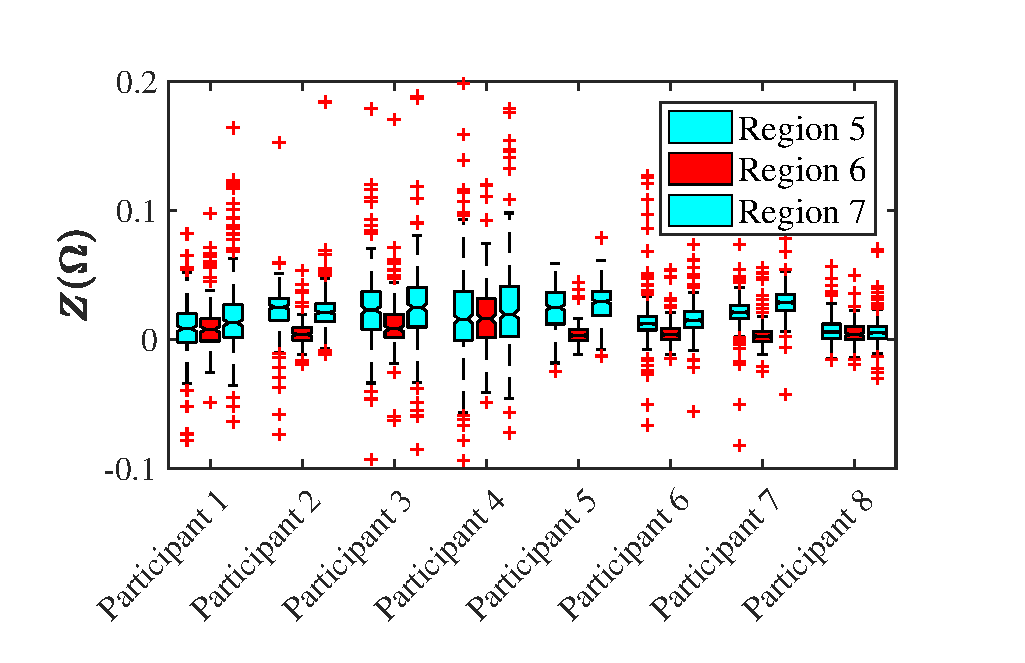
\includegraphics[width=0.48\textwidth, trim={0.5cm 0cm 1.5cm 0 cm}, clip]{figure_apa_7b}}%
	\hfill%
	\subcaptionbox{Change of amplitude of the waveform at point C.\label{fig:change_C_total}}
	[0.48\textwidth]{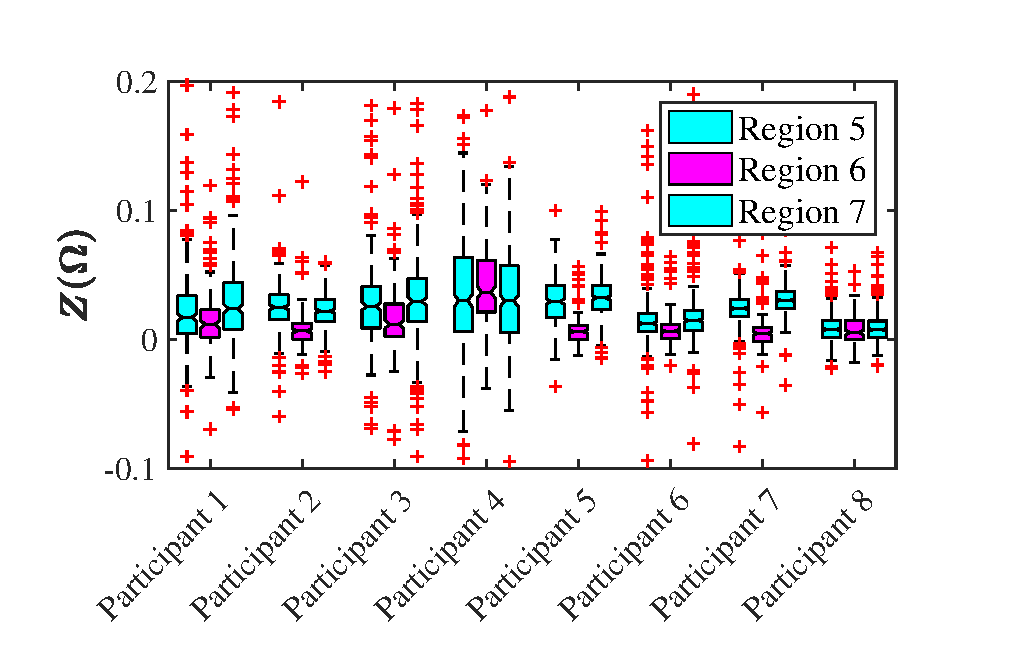
\includegraphics[width=0.48\textwidth, trim={0.5cm 0cm 1.5cm 0 cm}, clip]{figure_apa_7c}}%
	\null%
	\caption{Changes of the impedance peak values during baseline, total occlusion and return to baseline for points A,B and C.}
	\label{fig:iPG_change_points_total}
\end{figure*}

As shown in section \ref{section apa 2.3}, during total occlusion the APA amplitude was just a fraction of the baseline waveform.  Therefore, the $\Delta Z$ obtained to calculate the blood flow is a small number resulting in a low or null calculation. In this part of the analysis, the majority of the study members showed a decrease in blood circulation rate close to zero.  As is evident from table \ref{tbl:blood_flow_iPG_total}, almost all participants registered a significant drop in their blood flow calculation when the blockage was applied in region 6. Once more, Participant 4 displayed a unique response during the occlusion which median blood flow did not go close to zero. Above all, the median calculated blood flow during the arterial constriction was about \SI{0.3953}{1412}. One would expect a completely zero at this point as clearly there is not blood flow passing through the forearm. However, this measurement could be considered the error of equipment measurement caused by noise picked up by the device. 

After the tourniquet had been withdrawn, the blood flow recovered exponentially, portraying a fast return to baseline accompanied by an overshot peak and followed by settling towards a midpoint, as shown in figure \ref{fig:blood_flow_plethysmography}. This kind of shape is typical of a hyperaemia where the return of blood flow produces this overshot response, because of the fast filling of the vessels. The mean blood flow in the region 7 was about \SI{2.892(1332)}{\bfv}, which is very close to the original baseline region 5. In fact, the calculated flow reduction was about \SI{2.6}{\percent}. Though, it can be seen that participant 8 had an expected drop in the flow rate before the blockage and then an increase in the rate. This event is fascinating as these changes occurred in a blood flow bellow \SI{1}{\bfv}, but the device was able to notice the swing of blood flow rate. At this stage, the sensitivity for calculation of small changes in blood flow needs improvement because it detected flow values in other participants when there was no plethysmography signal. However, it is quite remarkable to see that the instrument is capable of detecting changes in the trend.


%%********************************** % Section 8.3 ******************************************
\section{Blood flow calculation from plethysmography signal}
\label{section apa 3}
So far the blood flow has been analysed from occlusive methods using the techniques described in section \ref{section occlusion 2}. However, these procedures require mechanical occlusion to produce an increase in volume within the forearm being measured. Nevertheless, sometimes this can be uncomfortable, especially when the applied pressure is above the systolic value or when the person just can not tolerate restriction of blood flow.

For these cases, analysing the waveform also provides information about the blood flow. The rush of blood into the vessel creates a small increase in volume within the limit of the potential electrodes which can be translated into a quantifiable blood flow. Having a device sensitive enough to detect these changes is crucial to provide an accurate estimation of the blood speed. As described in section \ref{section apa 3}, the waveform contained within the basal impedance was amplified by the device, achieving great detail.

In fact, different studies have demonstrated that it is possible to calculate blood flow from the analysis of the APA waveform \cite{corciova2011peripheral, costeloe1980continuous, brown1975impedance}. In this case, the change of impedance used to perform this calculation occurs between the foot of the wave and the systolic peak. This $\Delta Z$ is used to calculate blood flow by also applying Nyober's equation \ref{eq:Nyober}.

\begin{figure}[!htbp]
	\centering
	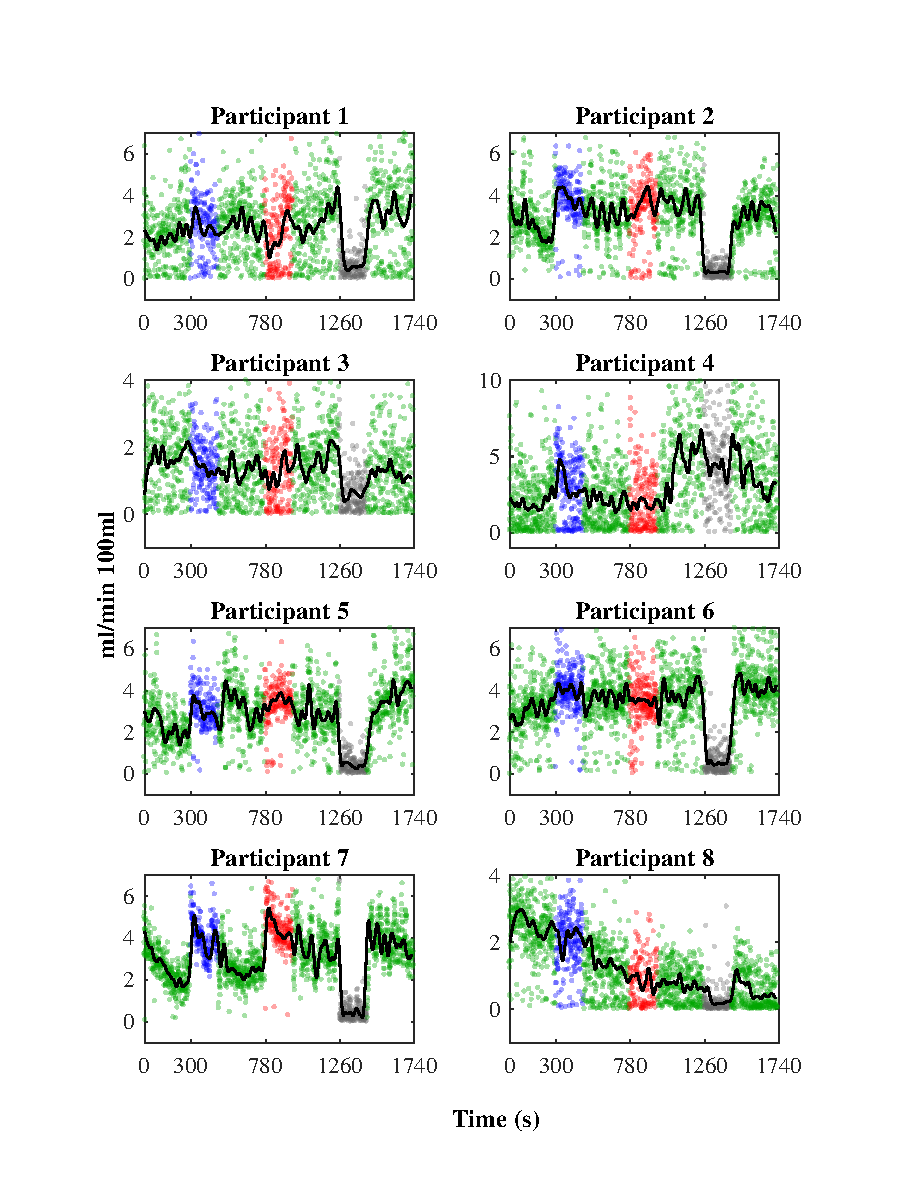
\includegraphics[keepaspectratio,trim={1.5cm 0cm 1.5cm 0 cm},clip]{figure_apa_8}
	\caption[Blood flow calculated from impedance plethysmography waveform at the time of the whole expetiment]{Blood flow calculated for all the participants during the experiment. Each dot represents the peak value of the waveform that has been converted into flow (\si{\bfv}). The green dotted area represent the baselines measurements (regions 1,3,5 and 7). The region 2 (venous occlusion) is represented by the blue dots, arterial occlusions (region 4) are in red and total occlusions (region 6) are in grey.}
	\label{fig:blood_flow_plethysmography}
\end{figure}

Figure \ref{fig:blood_flow_plethysmography} shows the blood flow derived from the amplitude of the systolic peak throughout the whole experimental session. Green dots show blood flow measurements during baseline readings (regions 1, 3, 5 and 6). The other colours indicate the venous occlusion in blue, partial arterial occlusion in red and total obstruction in grey. The dark line drawn above the signals corresponds to the smoothing of each measurement event using \textit{robust loess} method of the \textit{smooth} command in Matlab. Overseeing the amplitude transition in each region will help explain how the flow changes with each occlusive event. The value of the calculated blood flow shown in the same figure does not include the negative sign which represents the direction of flow relative to the potential electrodes.

As portrayed in the same figure, between each transition, in the middle of baseline and occlusion, some participants described clearly marked shifts in the calculated flow. In most participants, when venous occlusion occurred, the change between baseline and venous occlusion created a blood surge followed by a tendency for the flow to stabilise. It is worth noting that the increment of blood flow in participant 2 occurred before the venous occlusion. The reason for this is that the obstruction probably started before \SI{300}{\second} and the pressure applied to the arm was rather slow. There are other cases where the flow change occurred so fast that an entirely blank space can be seen connecting both events, as in participants 5 and 7. This situation, as opposed to participant 2, was more likely due to the cuff being inflated faster which did not allow a gradual but instead sudden change in flow. However, also, it could be related to a physiological response of the body like vasodilation response, where one reacts faster than others. Finally, participant 8 is an exception to this rule. This participant experienced a decrease in the calculated flow, followed by a stabilisation. A flow surge is not identifiable in this partaker.

Between venous occlusion and return to baseline in region 3, the cuff was rapidly deflated to restore blood flow to a normal condition. However, from the calculated data it can be seen that there are no extreme changes in blood flow between these two sections as soon as the blockage was released. As noted, in most participants except partakers 5 and 7, there are little changes between these two sections indicating that there is a slight change in blood flow. This action can be linked to a hyperaemic effect where as soon as the pressure of the cuff is released, the blood contained within the vessels of the forearm runs out to the upper part of the arm. After that, the blood flow tended to stabilise towards an average value.

Similarly, as between regions 1 and 2, the change between baseline (region 3) and partial arterial occlusion (region 4 - red colour) generated alterations in the calculated blood flow. Some participants, like partakers 6 and 7 showed a rapid increase in blood flow after the occlusion followed by settling in the blood velocity, where the latter is more notorious. Others like participants 1, 2, 3 and 5 showed a Gaussian bell-shaped flow during the occlusion. It is evident that their flow did not set in a mean value. The only ones that enacted different behaviour were participants 4 and 8, where not much change of blood is evident. However, it is notorious the continuous change of amplitude in participant 8 at this point which is contrary to the rest of participants.

The change between partial arterial occlusion (red section) and baseline had a similar effect as the one described for the release of pressure of venous blockage. Most of the participants showed a decrease in their blood flow, right after the cuff's pressure was released, possibly caused by a hyperaemic effect. At this point, one can note that participant 4 started to show random blood flow readings.

Total occlusion (grey dots) had an expected response in almost all the study members. When the blood flow was completely stopped, it was anticipated that its calculated value could tend to zero. In this case, the device was able to detect these changes. The only exception was participant 4 who again showed random results. At this point, it was to be expected that something wrong was happening with his measurements. Then, when the tourniquet was released, the blood flow returned in an exponential form and then set to an average value. In this case, the hyperaemic effect is more visible. It is worth noting that participant 8 showed a decline in blood flow measurements towards the midpoint of the test. This event agrees, with the partaker expressing not feeling very well at the end of the test. One can speculate it is a coincidence, or maybe the device was able to detect these physiological changes in him.

It seems evident that there is a blood surge when an occlusion in the blood circulation occurs from the impedance computation. Subsequently, the blood flow tends to stabilise at an average value. When the blockage is released, it seems that in some cases the flow tends to decrease and in others, there is no apparent change. The following sections will discuss the results of the change in median blood flow during each occlusive event.


%%********************************** % Section 8.3.1 ******************************************
\subsection{Blood flow change during venous occlusion}
\label{sectio results 3.1}
The following are the results of calculating the median blood flow between baseline in region 1, venous occlusion in region 2 and the return baseline after releasing the cuff's pressure in region 3. Once again, the result of the calculation is the absolute value, dropping the negative sign as this indicates the direction of the flow relative to the electrodes. Table \ref{tbl:blood_flow_iPG_venous} sums up the results obtained by flow measurement in the scale \si{\bfv}. The mean blood flow in region 1 was about \SI{2.283(0437)}{\bfv}. When the venous occlusion took place by inflating the cuff below diastolic value, the average blood flow calculated in region 2 was \SI{3.034(0938)}{\bfv}. It is easy to see that there was in increase of blood flow in approximately \SI{33}{\percent} during this part of the experiment. It seems that this increment in the blood flow could be due to a physiological response. It seems that there is a vasodilation process allowing extra blood to be retained in the venous circulation. However, study members 3 and 8 showed a decrease in their blood flow during this transition of about \SI{0.386(0011)}{\bfv}. The latter is not a surprise, as it was noted before, all his recordings started to go downwards from the beginning of the test. In the case of the participant 3, the obtained data seems not well distributed towards the mean. Therefore, there must be a significant number of outliers within its measurement making difficult extracting the real median blood flow. 

Clearly, there is a blood flow fall when the cuff's tension was released to return to the baseline signal. Indeed, six out of eight of the participants experienced a drop in their flow rate during this part of the experiment. The average blood flow for region 3 was approximately \SI{2.409(0885)}{\bfv}, which is equivalent to a \SI{5.5}{\percent} difference with the initial baseline at region 1. On the contrary, participants 1 and 5 did not experience this reduction of flow rate but a slight increase of less than \SI{0.09}{\bfv} or \SI{3.9}{\percent} increment when compared to the original reference signal.

\begin{table}[h]
	\caption{Mean blood flow calculated form the plethysmography wave for baseline, venous occlusion and return to baseline}
	\label{tbl:blood_flow_iPG_venous}
	\centering
	\begin{tabular}{l
				    *{3}{S[table-format=1.3]@{\,\( \pm \)\,}S[table-format=1.3]} %Format for Z+-std
					}
		\toprule
		& \multicolumn{2}{c}{\textbf{Region 1}}
		& \multicolumn{2}{c}{\textbf{Region 2}}
		& \multicolumn{2}{c}{\textbf{Region 3}}  \\
		& \multicolumn{2}{c}{\small{\si{[\bfv]}}}
		& \multicolumn{2}{c}{\small{\si{[\bfv]}}}
		& \multicolumn{2}{c}{\small{\si{[\bfv]}}} \\\midrule
	    Participant 1 & 2.046  & 1.772 & 2.688  & 1.638 & 2.710  & 1.481 \\
		Participant 2 & 2.516  & 1.185 & 3.766  & 1.161 & 3.119  & 1.252 \\
		Participant 3 & 1.794  & 1.282 & 1.416  & 0.796 & 1.325  & 1.260 \\
		Participant 4 & 1.811  & 2.032 & 3.296  & 2.010 & 1.748  & 1.959 \\
		Participant 5 & 2.033  & 1.082 & 3.024  & 0.947 & 3.110  & 1.277 \\
		Participant 6 & 3.054  & 1.289 & 4.019  & 1.146 & 3.566  & 1.330 \\
		Participant 7 & 2.555  & 0.930 & 3.993  & 0.924 & 2.483  & 0.827 \\
		Participant 8 & 2.461  & 0.874 & 2.068  & 0.901 & 1.207  & 0.729 \\
		\bottomrule
	\end{tabular}
\end{table}

%********************************** % Section 8.3.2 ******************************************
\subsection{Blood flow change during partial arterial occlusion}
\label{section apa 3.2}
The change of blood flow between the baseline (region 3) and partial arterial occlusion (region 4)  was not as evident as the response seen in the previous section, where most of the participants showed an increase in their calculated flow rate. Certainly, three out of eight participants reported an increase in their blood flow, whereas in the rest decreased.  In general, the average flow rate during baseline was \SI{2.408(0885)}{\bfv}. Later, during the partial arterial occlusion, the mean blood flow increased in just \SI{8.4}{\percent} to approximately \SI{2.612(1266)}{\bfv}. 

It is clear that the increase was not as notorious as the one seen all along venous occlusion. Indeed, participants (2, 5 and 7) showed an increment in blood flow with a centre of \SI{0.889(0925)}{\bfv}, especially the latter had the greatest change of blood flow. Conversely, the rest of the participants exhibited a small decrease in their blood flow with an average of \SI{-0.208(0180)}{\bfv}.

When the upper arm pressure was released in the region 5, it was expected that most of the participants would show a slump in their flow rate. However, this was not the case. The average blood flow at this stage was \SI{2.973}{1293}, which is equivalent to an increment of \SI{23}{\percent} from the baseline region 3. More in detail, three study members depicted a drop in their rate (5, 7 and 8) with an average of \SI{-0.618(0431)}{\bfv}. The rest of the study members showed an increase in their collected data of about \SI{0.948(1263)}{\bfv}. Notwithstanding, as previously described in this region, participant 4 showed random values entirely outlying the median obtained. At this stage, it is not possible to draw a clear conclusion whether an arterial occlusion would produce an increase or decrease of blood flow from the impedance measurement.

\begin{table}[h]
	\caption{Mean blood flow calculated form the plethysmography wave for baseline, partial arterial occlusion and return to baseline}
	\label{tbl:blood_flow_iPG_arterial}
	\centering
	\begin{tabular}{l
			*{3}{S[table-format=1.3]@{\,\( \pm \)\,}S[table-format=1.3]} %Format for Z+-std
		}
		\toprule
		& \multicolumn{2}{c}{\textbf{Region 3}}
		& \multicolumn{2}{c}{\textbf{Region 4}}
		& \multicolumn{2}{c}{\textbf{Region 5}}  \\
		& \multicolumn{2}{c}{\small{\si{[\bfv]}}}
		& \multicolumn{2}{c}{\small{\si{[\bfv]}}}
		& \multicolumn{2}{c}{\small{\si{[\bfv]}}} \\\midrule
	    Participant 1 & 2.710  & 1.481 & 2.251  & 1.689 & 2.977  & 1.791 \\
		Participant 2 & 3.119  & 1.252 & 3.486  & 1.399 & 3.537  & 1.492 \\
		Participant 3 & 1.325  & 1.260 & 1.299  & 1.025 & 1.647  & 1.132 \\
		Participant 4 & 1.748  & 1.959 & 1.665  & 1.895 & 4.832  & 7.032 \\
		Participant 5 & 3.110  & 1.277 & 3.454  & 0.994 & 2.841  & 1.225 \\
		Participant 6 & 3.566  & 1.330 & 3.417  & 1.197 & 3.866  & 1.558 \\
		Participant 7 & 2.483  & 0.827 & 4.441  & 1.001 & 3.389  & 1.050 \\
		Participant 8 & 1.207  & 0.729 & 0.882  & 0.864 & 0.693  & 0.537 \\
	\bottomrule
	\end{tabular}
\end{table}

%********************************** % Section 8.3.3 ******************************************
\subsection{Blood flow change during total occlusion}
\label{section apa 3.3}
The results obtained from total occlusion were quite close to the expected values.  The majority of the study participants showed a decrease in blood circulation rate close to zero.  As is evident from table \ref{tbl:blood_flow_iPG_total}, almost all participants showed a large drop in the blood flow measurement when the blockage was applied in region 6. Once more, Participant 4 displayed a completely unusual response during the occlusion. The values obtained were on average \SI{0.599(0224)}{\bfv} discarding data from partaker 4 \nknote{do you mean to staop and make this a new sentence or what?}. Clearly, the flow obtained did not reflect a zero blood flow. The calculated values correspond to the amplitude of the noise level captured by the device.

After the tourniquet had been withdrawn, the blood flow returned to baseline following an exponential shape \nknote{what shape?? do want another word?} in most of the participants as shown in figure \ref{fig:blood_flow_plethysmography}. The mean blood flow in the region 7 was about \SI{2.940(1276)}{\bfv}. However, it can be seen that participant 8 had an expected drop in the flow rate before the blockage and then an increase in value. This event is fascinating as these changes occurred in a blood flow bellow \SI{1}{\bfv} but the device was able to notice the swing of blood flow rate. At this stage, the sensitivity for calculation of small changes in blood flow needs improvement because it detected flow values in other participants when there was no plethysmography signal. However, it is quite remarkable to see that the instrument is capable of detecting changes in the trend.

\begin{table}[!htbp]
	\caption{Mean blood flow calculated form the plethysmography wave for baseline, total occlusion and return to normality}
	\label{tbl:blood_flow_iPG_total}
	\centering
	\begin{tabular}{l
			*{3}{S[table-format=1.3]@{\,\( \pm \)\,}S[table-format=1.3]} %Format for Z+-std
		}
		\toprule
		& \multicolumn{2}{c}{\textbf{Region 5}}
		& \multicolumn{2}{c}{\textbf{Region 6}}
		& \multicolumn{2}{c}{\textbf{Region 7}}  \\
		& \multicolumn{2}{c}{\small{\si{[\bfv]}}}
		& \multicolumn{2}{c}{\small{\si{[\bfv]}}}
		& \multicolumn{2}{c}{\small{\si{[\bfv]}}} \\\midrule
	    Participant 1 & 2.977  & 1.791 & 0.564  & 1.283 & 3.466  & 2.553 \\
		Participant 2 & 3.537  & 1.492 & 0.284  & 0.698 & 2.922  & 1.179 \\
		Participant 3 & 1.647  & 1.132 & 0.567  & 0.751 & 1.277  & 1.210 \\
		Participant 4 & 4.832  & 7.032 & 4.350  & 2.868 & 3.786  & 4.128 \\
		Participant 5 & 2.841  & 1.225 & 0.342  & 0.687 & 3.500  & 1.645 \\
		Participant 6 & 3.866  & 1.558 & 0.448  & 1.190 & 4.103  & 1.489 \\
		Participant 7 & 3.389  & 1.050 & 0.343  & 1.121 & 3.689  & 0.958 \\
		Participant 8 & 0.693  & 0.537 & 0.098  & 0.449 & 0.399  & 0.567 \\

		\bottomrule
	\end{tabular}
\end{table}

%%********************************** % Section 8.4 ******************************************
\section{Conclusions}
\label{section apa 4}
All the signals recorded were clear and offered an overview of what could happen during each occlusive event. The designed impedance device demonstrated that it was able to detect changes in basal impedance and plethysmography signals. Moreover, it seems that each occlusive event manifests a particular response like slope change in basal impedance and waveform amplitude at systolic and diastolic peaks during occlusions. \nknote{change this last sentence}

The other instruments were also able to detect changes during each event. For instance, the ultrasound device, referencing arterial flow, detected changes mostly in region 4 and 6 of the study. The LDF pointing towards microcirculatory flow was able to detect variations in flow in all the events. Moreover, it showed special sensitivity as soon as the flow was restored showing. \nknote{???} A clear hyperaemic response of the capillaries was portrayed in the signals. Red wavelength PPG was able to detect changes during all the events. The DC component of the signal detected changes during venous occlusion and partial arterial occlusion, but in total blockage it did not show a clear response. On the other hand, AC component portrayed variations to all occlusions showing sharp changes in amplitude during each occlusive episode.

%********************************** %Nomenclature found  *************************************
\nomenclature[z-IPP]{IPP}{Impedance plethysmography pulses}
